% !TeX program = lualatex
% SHR Converter 0.0.1 - user and technical manual. Generated by tools/build_manual.py; edit that, not this.
\documentclass[11pt,a4paper]{article}
\usepackage{fontspec}
\usepackage[margin=2.2cm]{geometry}
\usepackage{amsmath,amssymb}
\usepackage{booktabs,longtable,tabularx,array}
\usepackage{graphicx}
\usepackage{xcolor}
\usepackage{caption}
\usepackage{enumitem}
\usepackage[hidelinks,bookmarksnumbered,bookmarksopen,bookmarksopenlevel=2,
            pdftitle={SHR Converter 0.0.1 - Manual},
            pdfauthor={William W. Wallace},
            pdfsubject={Signal Hound Spike .shr to CSV and Veusz .vszh5},
            pdfkeywords={Signal Hound, Spike, SHR, CSV, Veusz, vszh5, spectrogram}]{hyperref}
\usepackage{bookmark}
\urlstyle{same}
\setlength{\LTcapwidth}{\linewidth}
\newcommand{\code}[1]{\texttt{#1}}
\title{SHR Converter 0.0.1\\[4pt]\large Signal Hound Spike \code{.shr} recordings to CSV and native Veusz documents\\
User and technical manual}
\author{William W. Wallace\\NRAO/GBO\\\code{wwallace@nrao.edu}}
\date{2026-10-28}
\begin{document}
\maketitle
\begin{center}
\begin{tabular}{ll}
\toprule
Program & Version\\
\midrule
\code{shr\_converter.py} (launcher) & 0.0.1\\
\code{shr\_converter\_gui.py} & 0.0.1\\
\code{shr\_converter\_core.py} & 0.0.1\\
\code{vszh5\_writer.py} & 0.0.20\\
py-shr-parser (reader) & 1.0.0\\
\bottomrule
\end{tabular}
\end{center}
\tableofcontents
\clearpage

\section{Overview}
Spike, Signal Hound's analyzer software, records sweeps to \code{.shr} files: a 472-byte file header, then
per sweep a 48-byte sweep header (time stamp, GPS latitude/longitude/altitude, ADC-overflow flag) and the
amplitudes as 32-bit floats \cite{r1},\cite{r2}. The SHR Converter reads these files with py-shr-parser
\cite{r1} and writes CSV tables and a native Veusz document (\code{.vszh5}) through the author's
\code{vszh5\_writer} \cite{r13}, optionally rendered by Veusz \cite{r10} to a bookmarked PDF and PNGs.
Everything is streamed in blocks, so memory is set by a RAM budget and not by the file, and the blocks run in
parallel worker processes, with the numerical part on the GPU when CuPy is present.

\section{Installation}
\begin{enumerate}[nosep]
\item \code{mamba env create -f environment.yml} --- Python 3.12; pip installs \code{requirements.txt}
      (py-shr-parser is on PyPI only).
\item \code{mamba activate shr-converter}
\item Optional: \code{mamba install -c conda-forge veusz} (or the Veusz installer) to open and render;
      \code{mamba install -c conda-forge cupy} for an NVIDIA GPU.
\item \code{python shr\_converter.py --selftest --gui-smoke} --- 38 engine checks and 11 GUI checks.
\item \code{python shr\_converter.py} starts the GUI. On Windows: \code{create\_environment.bat} once,
      then \code{run\_shr\_converter.bat} (files may be dropped on it) and \code{run\_selftest.bat}.
\end{enumerate}
The launcher imports nothing heavy at its top level: worker processes started with \emph{spawn} re-run the
main script's top level, and this keeps Qt (about 50~MB per process) out of them.

\section{The window}
\begin{figure}[htbp]\centering
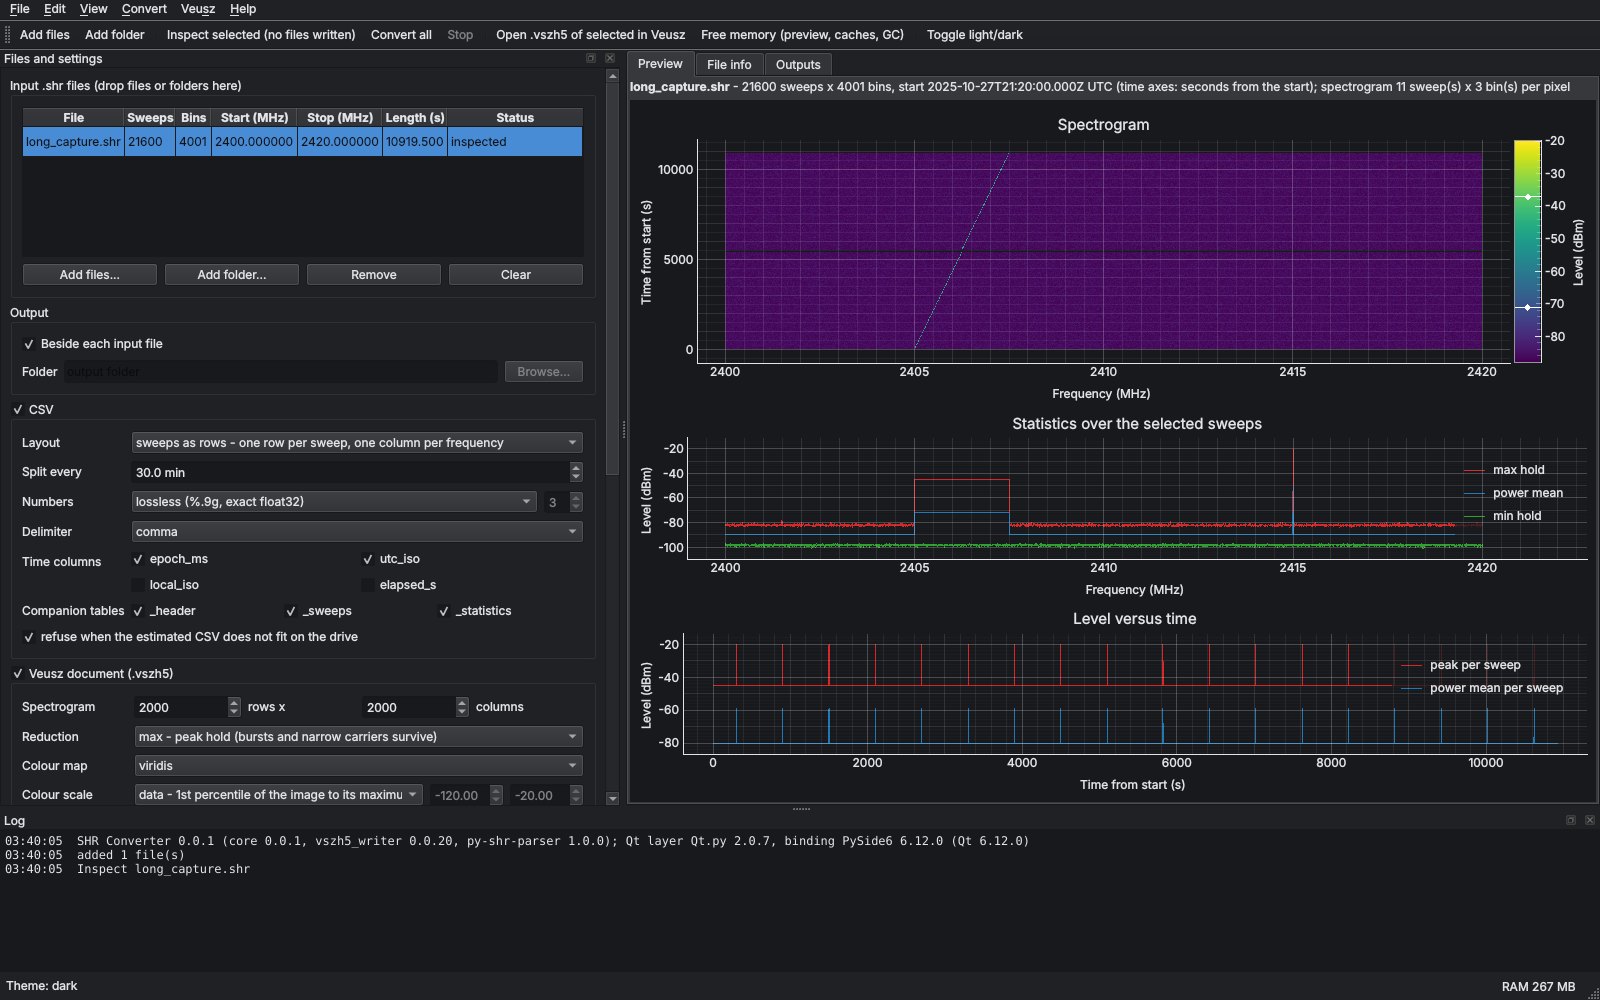
\includegraphics[width=\linewidth]{figures/gui_dark.png}
\caption{Dark theme, a synthetic 3-hour capture inspected: input list and settings (left), preview (centre), log (bottom).}
\end{figure}
\begin{figure}[htbp]\centering
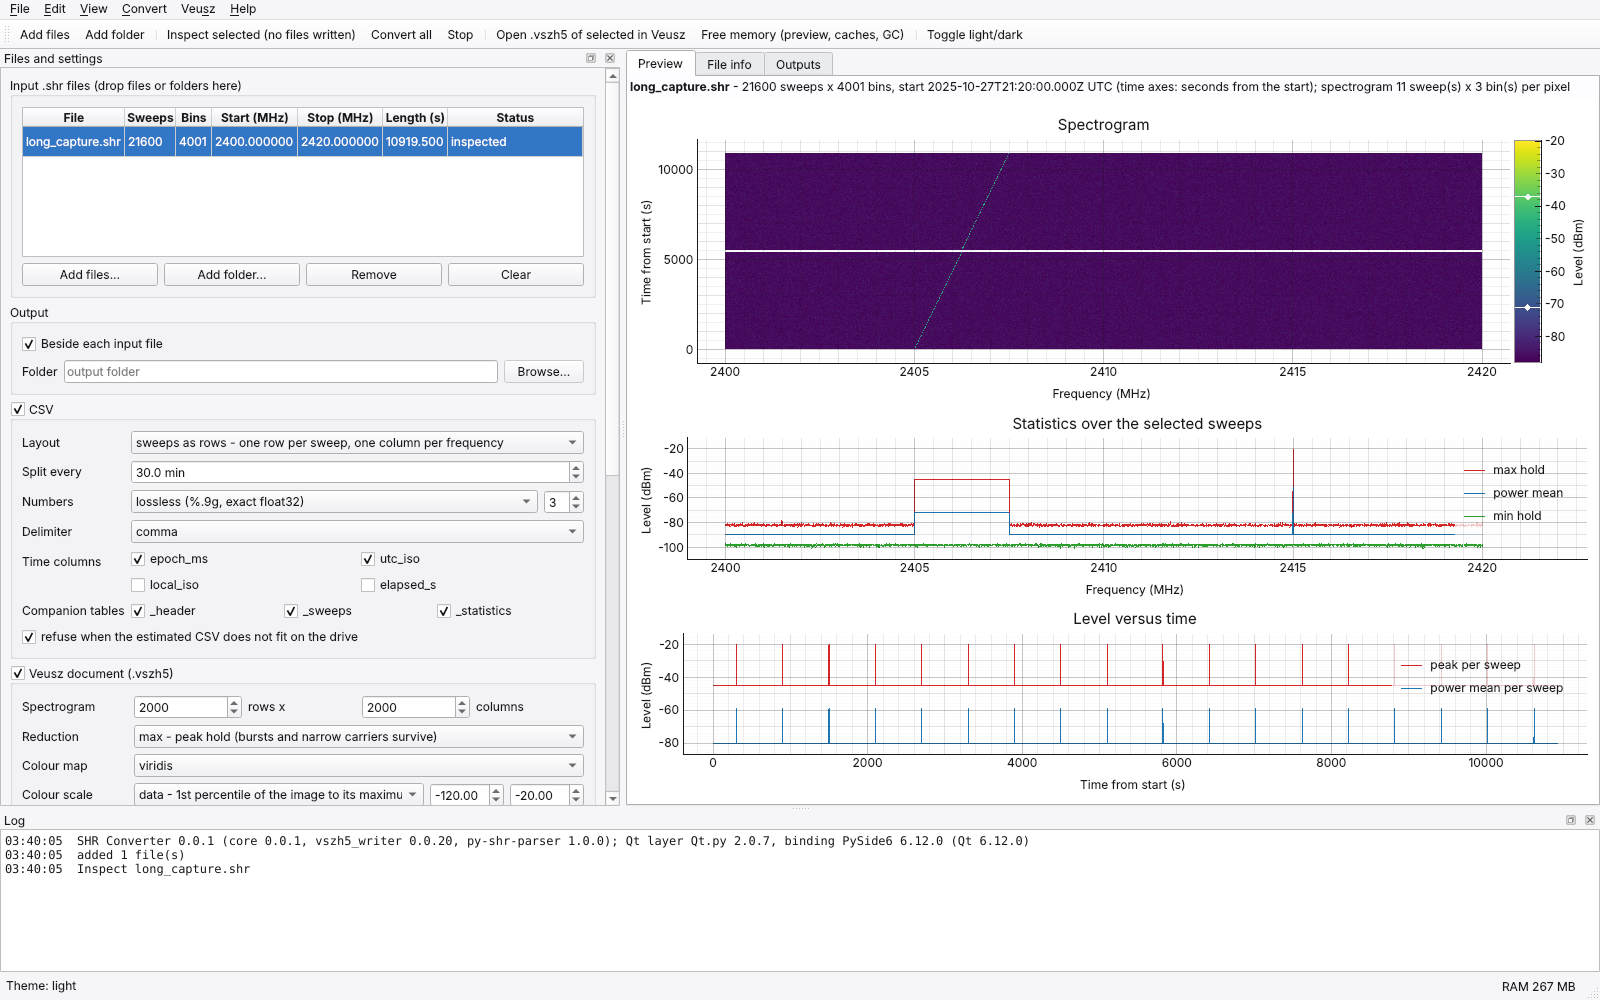
\includegraphics[width=\linewidth]{figures/gui_light.png}
\caption{Light theme (View > Theme, or Ctrl+T to toggle).}
\end{figure}
\subsection{Menus and keys}
\begin{description}[nosep,leftmargin=2.2cm,style=nextline]
\item[File] Add files (Ctrl+O), Add folder (Ctrl+Shift+O), Recent inputs, Remove (Del), Clear, Output folder,
      Open output folder (Ctrl+Shift+D), Save/Load settings (JSON), Save log, Quit.
\item[Edit] Copy file info, copy/clear log, \textbf{Free memory} (Ctrl+Shift+M).
\item[View] \textbf{Theme: System / Light / Dark}, toggle light/dark (Ctrl+T), auto-range (Ctrl+0), panels,
      toolbar, full screen (F11).
\item[Convert] Inspect (Ctrl+I), Convert all (F5), Convert selected (Shift+F5), Stop (Esc), Show plan (Ctrl+P),
      Self-test.
\item[Veusz] Open the \code{.vszh5} in Veusz (Ctrl+Shift+Z), Render to PDF/PNG (Ctrl+R), Open PDF.
\item[Help] Manual (F1), keyboard shortcuts, About (author, licence, every loaded version), About Qt.
\end{description}
\subsection{Workflow}
\begin{enumerate}[nosep]
\item Add files. Each header is read at once (sweeps, bins, span, length); notes report cut-short recordings.
\item \textbf{Inspect} runs the complete statistics pass without writing any file --- the same code as
      Convert --- and shows the preview. The \emph{File info} tab shows the plan
      (Figure~\ref{fig:info}).
\item \textbf{Convert}: one worker pool serves the whole batch; each file's preview arrives when it is
      done. \textbf{Stop} ends after the current block and deletes that file's partial outputs.
\end{enumerate}
\begin{figure}[htbp]\centering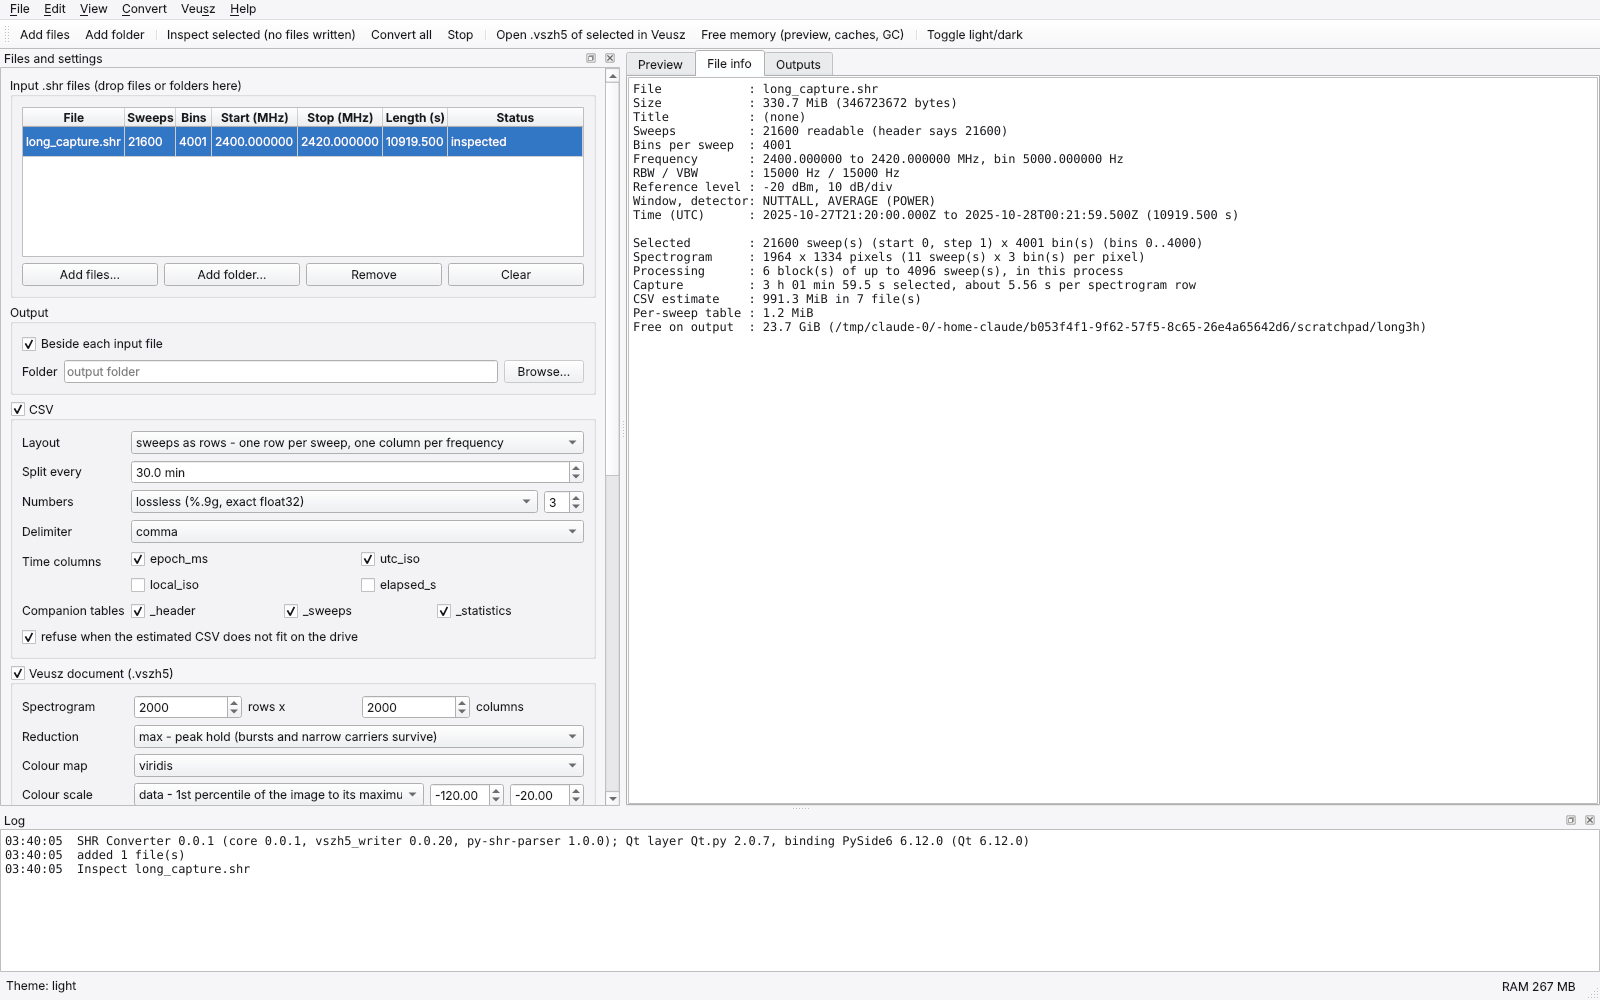
\includegraphics[width=\linewidth]{figures/gui_fileinfo.png}
\caption{File info: header, plan, CSV estimate, seconds per spectrogram row and free disk space.}\label{fig:info}
\end{figure}

\section{Outputs}
\subsection{CSV}
\begin{description}[nosep,leftmargin=3.6cm,style=nextline]
\item[\code{sweeps\_as\_rows}] one row per sweep: index, time columns, GPS, overflow, then one column per
      frequency (header: the bin frequencies in Hz). The default.
\item[\code{frequencies\_as\_rows}] one row per bin: frequency, then one column per sweep. Needs every
      selected sweep of a column block at once, so the file is read once per block (the plan says how often).
\item[\code{long}] one row per sample: index, time columns, frequency, amplitude.
\end{description}
Companion tables: \code{\_header.csv} (every header field with its unit, derived values, CSV parts with their
time spans, versions), \code{\_sweeps.csv} (per sweep: time, GPS, overflow, peak, peak frequency, power mean)
and \code{\_statistics.csv} (per bin: max hold, min hold, power mean, dB mean, standard deviation, count).
Files are written to private \code{.part} names and published only when complete; a CSV that another program
holds open (Excel on Windows) is kept under a time-stamped name. Excel's limits (16\,384 columns,
1\,048\,576 rows \cite{r6}) are reported by the plan.

\subsection{Veusz document}
\begin{longtable}{ll}
\toprule
\textbf{Page} & \textbf{Title (PDF bookmark)}\\
\midrule
\endhead
\texttt{spectrogram} & Spectrogram\\
\texttt{statistics} & Spectrum statistics\\
\texttt{selected\_\allowbreak{}sweeps} & Selected sweeps\\
\texttt{level\_\allowbreak{}vs\_\allowbreak{}time} & Level versus time\\
\texttt{gps\_\allowbreak{}track} & GPS track\\
\texttt{file\_\allowbreak{}header} & File header\\
\bottomrule
\end{longtable}
\begin{figure}[htbp]\centering
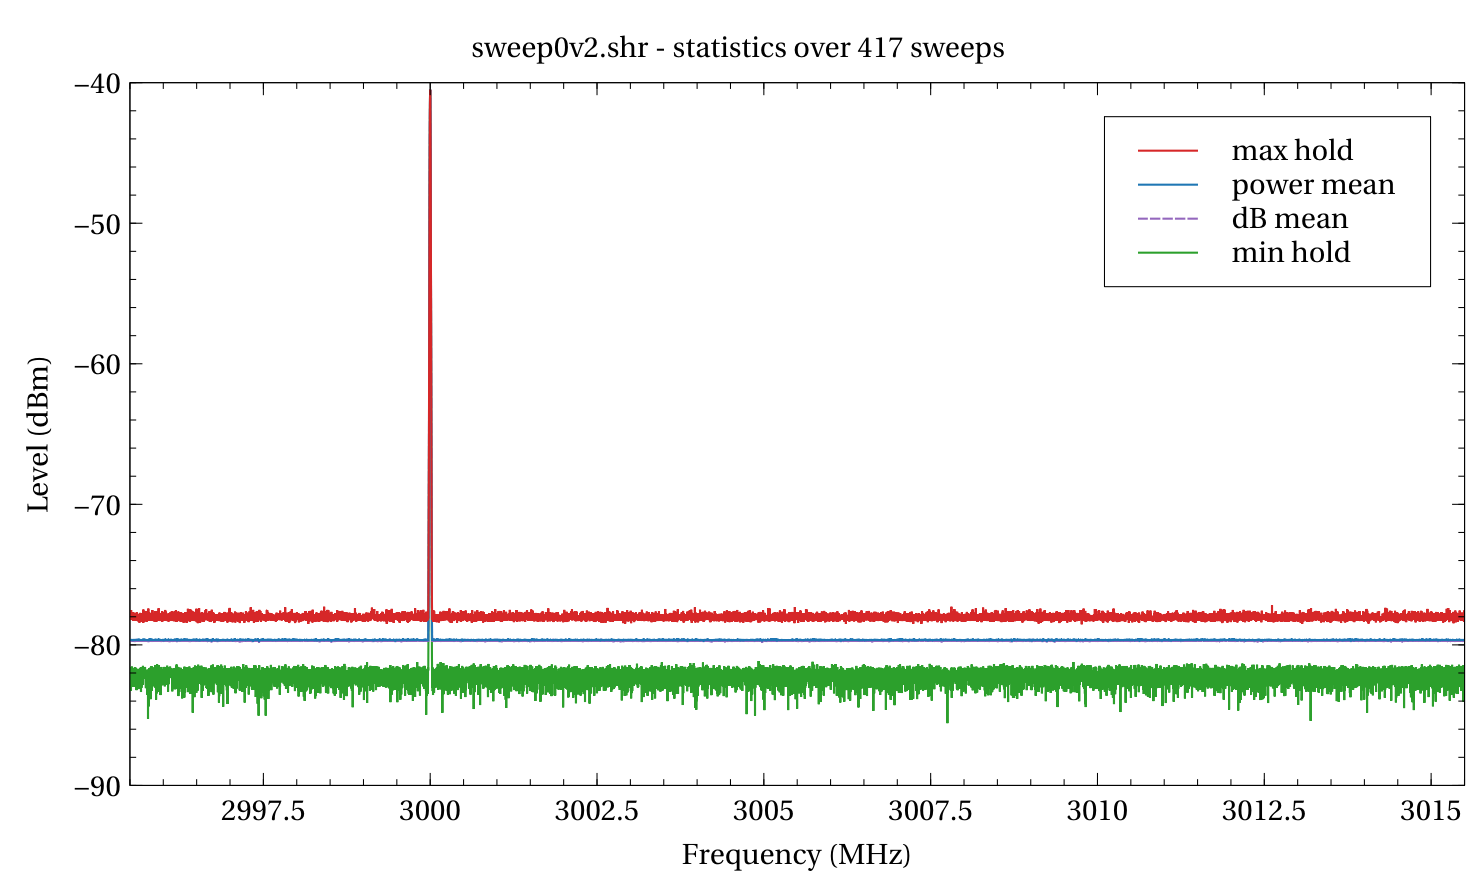
\includegraphics[width=\linewidth]{figures/veusz_statistics_sweep0v2.png}
\caption{Statistics page of Spike's own test file sweep0v2.shr (417 sweeps): max hold, power mean, dB mean, min hold.}
\end{figure}
\begin{figure}[htbp]\centering
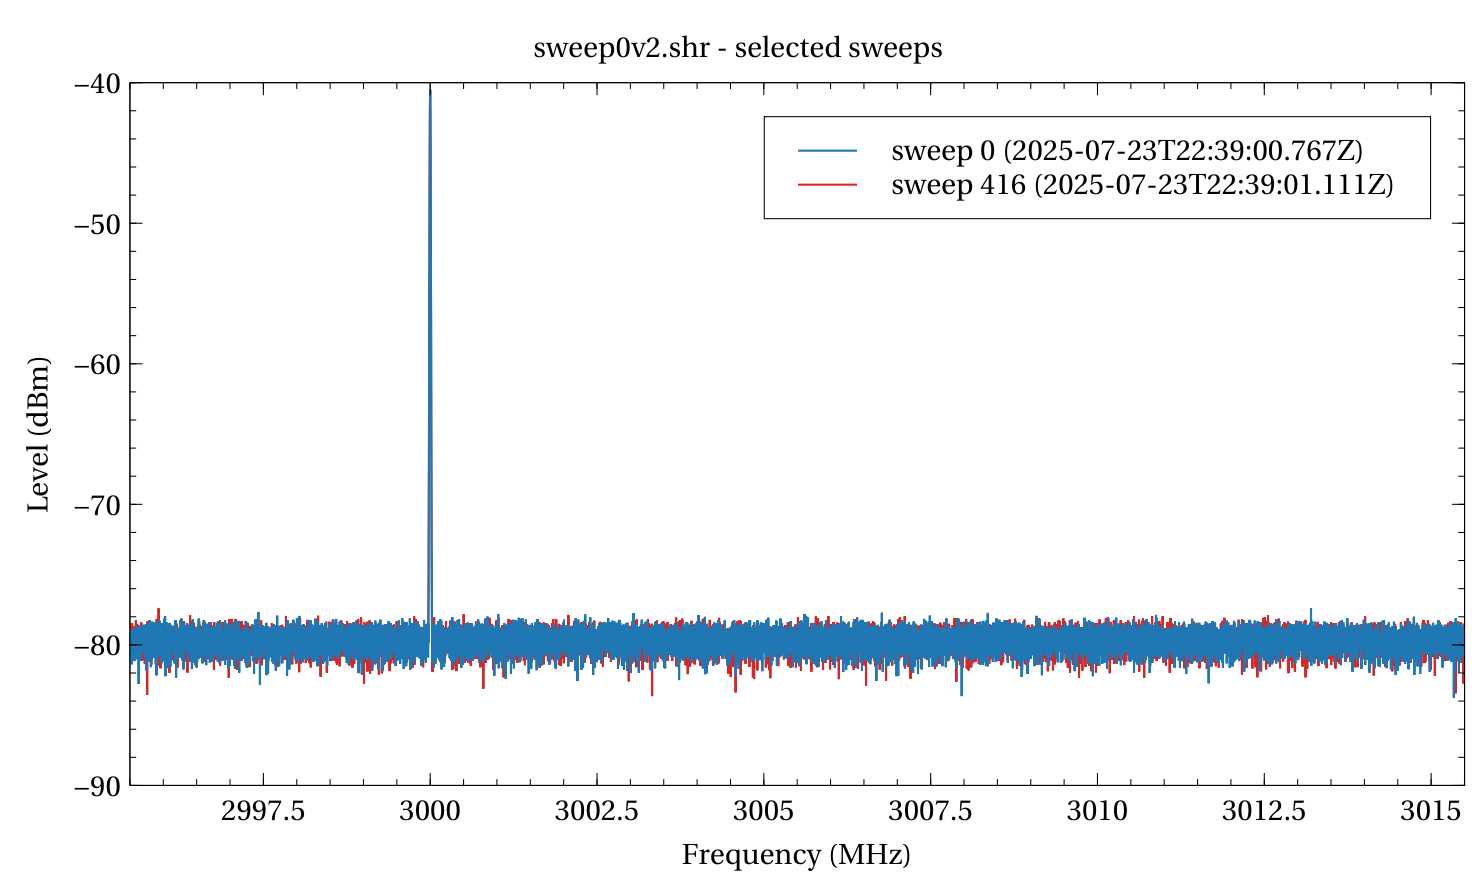
\includegraphics[width=\linewidth]{figures/veusz_selected_sweeps_sweep0v2.png}
\caption{Selected-sweeps page: first and last sweep (the peak sweep is the first here).}
\end{figure}

\section{Statistics and their derivations}
Let $x_k(f)$ be the level of bin $f$ in sweep $k$, $k=1\ldots N$.
\subsection{Frequency of a bin}
\begin{equation}f_i = f_0 + i\,\Delta f,\qquad f_0=\code{first\_bin\_freq\_hz},\ \Delta f=\code{bin\_size\_hz}.\end{equation}
This is the file header's definition, also used by py-shr-parser for the peak frequency. Its plotting helpers
use $\mathrm{linspace}(f_c-S/2, f_c+S/2, n)$ instead; on \code{sweep0v2.shr}
($\Delta f = 1220.703125$~Hz, $n=16\,386$, $S=20$~MHz) the two differ by up to one bin at the top, because
$(n-1)\,\Delta f = 20.0012$~MHz $\neq S$.
\subsection{Power mean, dB mean and the 2.51 dB bias}
\begin{align}
\bar P(f) &= 10\log_{10}\!\Big(\frac1N\sum_{k=1}^{N}10^{x_k(f)/10}\Big)\quad[\mathrm{dBm}],\\
\bar L(f) &= \frac1N\sum_{k=1}^{N}x_k(f)\quad[\mathrm{dBm}].
\end{align}
For noise the dB mean reads low \cite{r4}. With a Rayleigh envelope the power $p$ is exponential with mean
$\mu$, $\rho(p)=\mu^{-1}e^{-p/\mu}$, and with $u=p/\mu$
\begin{equation}
\mathrm{E}[\ln p]=\ln\mu+\int_0^\infty \ln u\,e^{-u}\,\mathrm du=\ln\mu+\Gamma'(1)=\ln\mu-\gamma,
\end{equation}
so
\begin{equation}
\mathrm{E}[10\log_{10}p]-10\log_{10}\mu=-\frac{10\,\gamma}{\ln 10}=-2.5068~\mathrm{dB},
\qquad \gamma=0.5772156649\ldots
\end{equation}
(a $10^7$-sample simulation gave $-2.5067$~dB). The converter therefore reports both: the power mean is the
physical mean power, the dB mean matches Spike's log averaging.
\subsection{mV recordings}
\begin{equation}V_\mathrm{rms}(f)=\sqrt{\frac1N\sum_k x_k(f)^2}\quad[\mathrm{mV}].\end{equation}
\subsection{Standard deviation from running sums}
\begin{equation}s^2=\frac{S_2-S_1^2/N}{N-1},\qquad S_1=\sum_k x_k,\ S_2=\sum_k x_k^2 .\end{equation}
In float64 the cancellation error is about $\varepsilon\,\bar x^2/s^2\approx 10^{-16}\times 80^2/2^2\approx
2\times10^{-13}$ (relative), negligible for dBm levels.
\subsection{Exact merging of blocks}
Each block returns $\max$, $\min$, $S_1$, $S_2$, $\sum 10^{x/10}$ and $N$ per bin; the file's values follow
exactly: maxima of maxima, minima of minima, sums of sums, e.g.
$\bar P_{A\cup B}=10\log_{10}\big((\Sigma_A+\Sigma_B)/(N_A+N_B)\big)$. Parallel and serial conversions give
identical results (self-test).
\subsection{Spectrogram pixels}
A pixel covers $n_r$ sweeps $\times$ $n_c$ bins. Peak hold is the block maximum; the power mean is
\begin{equation}
\bar P_{ij}=10\log_{10}\Big(\frac{1}{n_r n_c}\sum_{k\in r_i}\sum_{f\in c_j}10^{x_k(f)/10}\Big)
=10\log_{10}\Big(\frac{1}{n_r}\sum_{k\in r_i}\Big[\frac1{n_c}\sum_{f\in c_j}10^{x_k(f)/10}\Big]\Big),
\end{equation}
computed as the column mean per sweep, then summed over the sweeps of the row (exact, since every sweep of a
row has the same $n_c$). A row may span two worker blocks; its partial sums are added by the main process.
\subsection{Lossless numbers}
Binary32 has $p=24$ significand bits; a decimal string round-trips with \cite{r5},\cite{r12}
\begin{equation}d=\lceil p\log_{10}2\rceil+1=\lceil 7.22\rceil+1=9\end{equation}
significant digits, hence \code{\%.9g}. Every value of every layout was compared with py-shr-parser bit for bit.

\section{Time axes and the even grid}
Time stamps are milliseconds since 1970 UTC from the recording PC's clock \cite{r2}. The \code{.vszh5}
time axis is UTC or local date/time, elapsed seconds or sweep index (\code{auto}: date/time for captures of
60~s or more). Spectrogram rows are put on an even grid by \code{vszh5\_writer.regularize\_rows}: the step is
fitted over the whole span, $\Delta=(c_{\mathrm{last}}-c_0)/s_{\mathrm{last}}$ with slots
$s_k=\mathrm{round}((c_k-c_0)/\Delta)$; rows that already lie within $\Delta/4$ of the grid are kept; pauses
become blank (NaN) rows; crowded time stamps are spread evenly. Veusz draws images with uneven axes through a
non-linear path: on a 3-hour spectrogram 30.3~s and 3.2~GB, against 2.7~s and 0.31~GB on the even grid.

\section{Long captures}
\begin{itemize}[nosep]
\item \textbf{CSV split by time}: \code{\_part001.csv}, \ldots, one per N minutes of recording, each with the
      header line; slices follow the running maximum of the time stamps, so a clock step back never sends a
      sweep to an earlier file.
\item \textbf{Disk check}: the CSV size is estimated (lossless: $\approx 12$ bytes per value) and the
      conversion refuses to start when the drive cannot hold it.
\item \textbf{Per-sweep table}: 57 bytes per sweep, memory-mapped from a private temporary folder when larger
      than a quarter of the RAM budget.
\item \textbf{Thinned series}: level versus time and GPS in the \code{.vszh5} are reduced to
      \code{time\_series\_max\_points} (100\,000) --- peak hold for the peak, power mean for the band level,
      the frequency of the strongest sweep, any overflow --- so a single burst is never averaged away.
\item \textbf{Time per row}: 2000 rows over 3~h is 5.4~s per row; the plan states it.
\end{itemize}
\begin{figure}[htbp]\centering
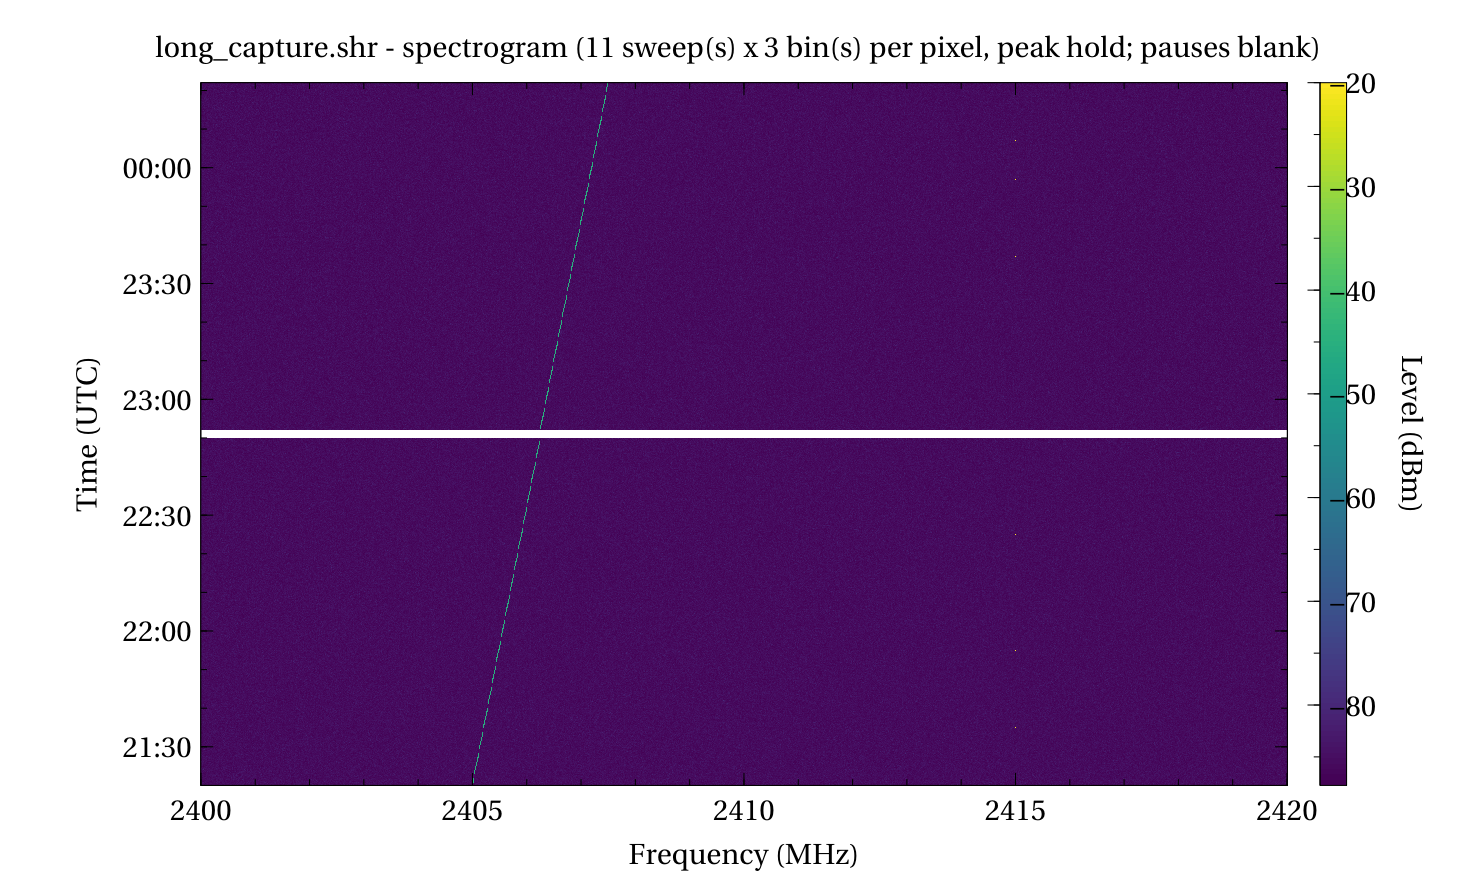
\includegraphics[width=\linewidth]{figures/veusz_spectrogram_3h.png}
\caption{Synthetic 3-hour capture: drifting carrier, a 2 ms burst every 10 min at 2415 MHz, a 2-minute pause (blank band).}
\end{figure}
\begin{figure}[htbp]\centering
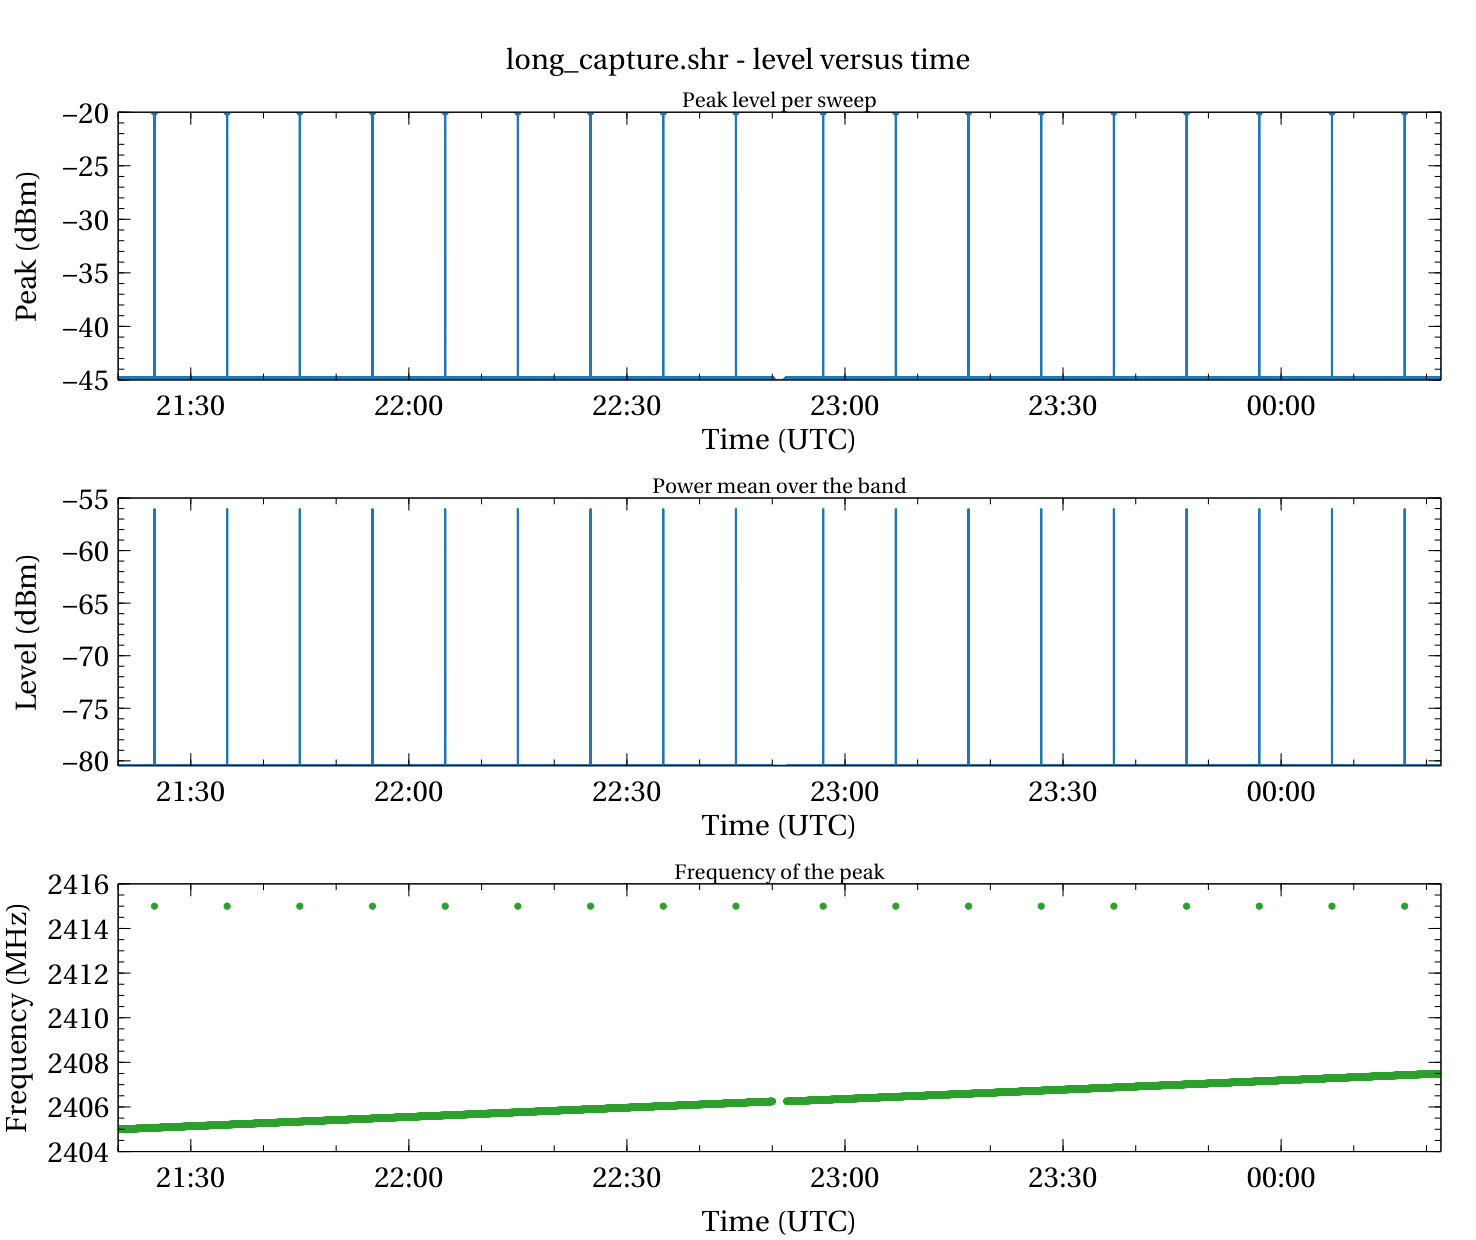
\includegraphics[width=\linewidth]{figures/veusz_level_vs_time_3h.png}
\caption{Level versus time of the same capture: every burst present, the pause visible.}
\end{figure}

\section{Performance, parallelism, GPU and memory}
\begin{itemize}[nosep]
\item Blocks of sweeps are read, formatted and reduced in worker processes (\emph{spawn}, never fork a GUI),
      at most $2\times$workers blocks in flight, merged in order \cite{r8}. Default workers: CPUs $-1$
      (at most 61 on Windows).
\item Block size: $B=\lfloor (M-M_\mathrm{stats})/(s\,n_c\,\beta)\rfloor$ with budget $M$, $s=2w+1$ slots,
      $n_c$ bins and $\beta$ bytes per sample in flight (30 for \code{sweeps\_as\_rows}); the statistics
      work in sub-blocks of 2~M samples, so their float64 temporaries do not grow with the block.
\item GPU: CuPy \cite{r9} runs the statistics and spectrogram reduction per sub-block; any GPU error repeats
      the block on the CPU (tested with a stand-in). Text formatting stays on the CPU.
\item Edit $>$ Free memory: garbage collection, CuPy pools, \code{malloc\_trim} / \code{EmptyWorkingSet};
      previews are pickled to disk, one in memory.
\end{itemize}
\begin{longtable}{p{6.2cm}p{4.2cm}rr}
\caption{Measured with tests/long\_capture\_check.py and tests/memory\_check.py (docs/validation).}\\
\toprule
\textbf{Case (2 CPU cores, no GPU)} & \textbf{Data} & \textbf{Time} & \textbf{Peak memory}\\
\midrule
\endhead
3 h, 2 sweeps/s x 4001 bins, 2 workers, with the Veusz PDF/PNG render & 331 MiB to 981 MiB CSV, 7 files & 25.8 s & 879 MiB\\
3 h, 50 sweeps/s x 512 bins (540 000 sweeps), 2 workers & 1.1 GiB to CSV (2 decimals) & 52.8 s & 526 MiB\\
3000 x 65 536 bins, RAM budget 256 MB, 2 workers & 750 MiB to 2.2 GiB CSV & 41.4 s & 418 MiB\\
\bottomrule
\end{longtable}

\section{Robustness}
\begin{itemize}[nosep]
\item py-shr-parser raises \code{ShrFileParserWarning} when the size does not match the header and leaves
      the file open; the converter reads up to the last complete sweep (header count 0 is replaced by the
      sweeps present) and says so \cite{r2}.
\item Every output is written to a private \code{.part} and published atomically; Stop, an error or a
      refused disk check leaves no partial file.
\item Published files get the usual permissions (writer 0.0.20 fix of the 0600 mode).
\end{itemize}

\section{Command line}
\code{python shr\_converter.py --cli [options] files-or-folders}
\begin{longtable}{p{4.6cm}p{11cm}}
\toprule
\textbf{Option} & \textbf{Meaning}\\
\midrule
\endhead
\texttt{inputs} & .shr files or folders (folders: every *.shr inside)\\
\texttt{-o, --output-dir} & output folder (default: beside each input)\\
\texttt{--no-csv} & do not write the CSV files\\
\texttt{--layout} & CSV layout: sweeps\_as\_rows (default), frequencies\_as\_rows or long\\
\texttt{--fixed} & fixed decimals instead of lossless \%.9g\\
\texttt{--delimiter} & CSV delimiter: comma (default), semicolon or tab\\
\texttt{--time-columns} & comma list of epoch\_ms, utc\_iso, local\_iso, elapsed\_s\\
\texttt{--no-companions} & skip \_header/\_sweeps/\_statistics.csv\\
\texttt{--split-minutes} & new CSV file every N minutes of recording (0 = one file)\\
\texttt{--no-disk-check} & do not refuse when the CSV may not fit\\
\texttt{--no-vszh5} & do not write the Veusz document\\
\texttt{--image-size} & maximum spectrogram ROWSxCOLUMNS\\
\texttt{--reduction} & spectrogram pixels: max (peak hold, default), power\_mean or min\\
\texttt{--colormap} & Veusz colour map, e.g. viridis, magma, heat\\
\texttt{--z} & data | reference | veusz | MIN,MAX\\
\texttt{--time-axis} & auto (date/time from 60 s on), utc, local, elapsed or index\\
\texttt{--sweeps-to-plot} & selected-sweeps page: first,last,peak and/or sweep indices\\
\texttt{--render} & render PDF (bookmarked) and PNG with Veusz\\
\texttt{--png} & PNG pages when rendering: first (default), all or none\\
\texttt{--veusz} & Veusz program (else VEUSZ\_EXE, PATH, usual folders)\\
\texttt{--sweeps} & sweep selection START:STOP:STEP (STOP exclusive)\\
\texttt{--freq} & frequency range FMIN:FMAX in MHz\\
\texttt{-j, --workers} & worker processes (0 = CPUs - 1)\\
\texttt{--ram-mb} & RAM budget for blocks\\
\texttt{--compute} & statistics on auto (CuPy GPU when present), cpu or gpu (falls back to CPU)\\
\texttt{--series-points} & maximum points of the level-vs-time and GPS series in the .vszh5\\
\texttt{--sweep-table} & per-sweep table in RAM or memory-mapped on disk (auto: by size)\\
\texttt{--info} & print header, plan and notes only\\
\texttt{--selftest} & run the self-test and exit\\
\texttt{--real-file} & also check this real .shr in the self-test\\
\texttt{--version} & show program's version number and exit\\
\bottomrule
\end{longtable}

\section{vszh5\_writer 0.0.20}
Two releases were both numbered 0.0.18: the R\&S FSP logger 0.9.0 (render fixes) and the AB Power Meter
Monitor 1.6.0 (\code{VeuszAppender}); 0.0.19 grew from the latter. 0.0.20 joins them and adds the 0600 file-mode
fix, \code{png\_background}, date-axis images, \code{block\_reduce} and \code{regularize\_rows}. Every public
signature of 0.0.5, 0.0.10, both 0.0.18 and 0.0.19 is unchanged (checked by machine).
\begin{longtable}{p{4.4cm}p{5.4cm}p{6cm}}
\toprule
\textbf{Program} & \textbf{Own suite with 0.0.20} & \textbf{Note}\\
\midrule
\endhead
R\&S FSP logger 0.9.0 & 44/44 (PyQt5, PySide6; Veusz 3.6.2, 4.2.1) & update the About test's expected version 0.0.18 -\textgreater{} 0.0.20\\
AB Power Meter Monitor 1.7.0 & 45/45, real renders & none\\
SA Time Stability Tools 0.0.3 & 7/7 and 22/22 in Veusz 4.2.1 & none\\
QuickSyn package 0.0.10 & 44 pass, 3 pinned checks fail & same with 0.0.19: version string and pre-0.0.15 temporary name\\
\bottomrule
\end{longtable}

\section{Verification}
\code{--selftest}: 38 checks (every CSV layout bit-exact with 1 and 2 workers; statistics, spectrogram and
sub-block merging against direct NumPy; cut-short files; mV; GPU stand-in and fallback; split, disk check,
disk-mapped table, thinning; locked file; cancel). \code{--gui-smoke}: 11 offscreen GUI checks including real
worker processes. \code{pytest tests}: 28 tests with 30 sub-tests, real renders in Veusz 3.6.2 and 4.2.1 and
Spike's own \code{sweep0v2.shr}. Logs: \code{docs/validation}.

\section{Data gaps}
\begin{longtable}{p{4.2cm}p{8.6cm}l}
\toprule
\textbf{Item} & \textbf{Status} & \textbf{Confidence}\\
\midrule
\endhead
Real Spike files & sweep0v2.shr (v2, dBm) read bit-exactly & High\\
mV recordings & synthetic only & Medium\\
Title encoding & UTF-16LE if it looks like it, else UTF-8; no titled file seen & Medium\\
Channelized recordings & read as stored, not interpreted & Unknown\\
GPU & stand-in only; no CUDA device here & Medium\\
Windows & designed for it, tested on Linux & Medium\\
\bottomrule
\end{longtable}

\appendix
\section{Options (ConvertOptions) and their defaults}
\begin{longtable}{p{5.6cm}p{9.6cm}}
\toprule
\textbf{Field} & \textbf{Default}\\
\midrule
\endhead
\texttt{output\_\allowbreak{}dir} & \texttt{""}\\
\texttt{write\_\allowbreak{}csv} & \texttt{True}\\
\texttt{csv\_\allowbreak{}layout} & \texttt{"sweeps\_\allowbreak{}as\_\allowbreak{}rows"}\\
\texttt{csv\_\allowbreak{}number\_\allowbreak{}format} & \texttt{"lossless"}\\
\texttt{csv\_\allowbreak{}decimals} & \texttt{3}\\
\texttt{csv\_\allowbreak{}delimiter} & \texttt{"comma"}\\
\texttt{csv\_\allowbreak{}time\_\allowbreak{}columns} & \texttt{('epoch\_\allowbreak{}ms', 'utc\_\allowbreak{}iso')}\\
\texttt{csv\_\allowbreak{}header\_\allowbreak{}table} & \texttt{True}\\
\texttt{csv\_\allowbreak{}sweeps\_\allowbreak{}table} & \texttt{True}\\
\texttt{csv\_\allowbreak{}statistics\_\allowbreak{}table} & \texttt{True}\\
\texttt{csv\_\allowbreak{}split\_\allowbreak{}minutes} & \texttt{0.0}\\
\texttt{check\_\allowbreak{}disk\_\allowbreak{}space} & \texttt{True}\\
\texttt{write\_\allowbreak{}vszh5} & \texttt{True}\\
\texttt{vszh5\_\allowbreak{}compress} & \texttt{True}\\
\texttt{image\_\allowbreak{}max\_\allowbreak{}rows} & \texttt{2000}\\
\texttt{image\_\allowbreak{}max\_\allowbreak{}columns} & \texttt{2000}\\
\texttt{image\_\allowbreak{}reduction} & \texttt{"max"}\\
\texttt{colormap} & \texttt{"viridis"}\\
\texttt{z\_\allowbreak{}mode} & \texttt{"data"}\\
\texttt{z\_\allowbreak{}min} & \texttt{-120.0}\\
\texttt{z\_\allowbreak{}max} & \texttt{-20.0}\\
\texttt{time\_\allowbreak{}axis} & \texttt{"auto"}\\
\texttt{selected\_\allowbreak{}sweeps} & \texttt{"first,last,peak"}\\
\texttt{stats\_\allowbreak{}max\_\allowbreak{}points} & \texttt{200000}\\
\texttt{time\_\allowbreak{}series\_\allowbreak{}max\_\allowbreak{}points} & \texttt{100000}\\
\texttt{page\_\allowbreak{}spectrogram} & \texttt{True}\\
\texttt{page\_\allowbreak{}statistics} & \texttt{True}\\
\texttt{page\_\allowbreak{}selected\_\allowbreak{}sweeps} & \texttt{True}\\
\texttt{page\_\allowbreak{}level\_\allowbreak{}vs\_\allowbreak{}time} & \texttt{True}\\
\texttt{page\_\allowbreak{}gps} & \texttt{True}\\
\texttt{page\_\allowbreak{}header} & \texttt{True}\\
\texttt{render} & \texttt{False}\\
\texttt{render\_\allowbreak{}png} & \texttt{"first"}\\
\texttt{render\_\allowbreak{}dpi} & \texttt{150}\\
\texttt{veusz\_\allowbreak{}exe} & \texttt{""}\\
\texttt{sweep\_\allowbreak{}start} & \texttt{0}\\
\texttt{sweep\_\allowbreak{}stop} & \texttt{0}\\
\texttt{sweep\_\allowbreak{}step} & \texttt{1}\\
\texttt{freq\_\allowbreak{}min\_\allowbreak{}hz} & \texttt{0.0}\\
\texttt{freq\_\allowbreak{}max\_\allowbreak{}hz} & \texttt{0.0}\\
\texttt{workers} & \texttt{0}\\
\texttt{ram\_\allowbreak{}budget\_\allowbreak{}mb} & \texttt{1024}\\
\texttt{compute} & \texttt{"auto"}\\
\texttt{sweep\_\allowbreak{}table\_\allowbreak{}storage} & \texttt{"auto"}\\
\texttt{flush\_\allowbreak{}after\_\allowbreak{}file} & \texttt{True}\\
\bottomrule
\end{longtable}
\section{File-header fields}
\begin{longtable}{p{4.4cm}p{2.2cm}p{8.6cm}}
\toprule
\textbf{Field} & \textbf{Unit} & \textbf{Meaning}\\
\midrule
\endhead
\texttt{signature} &  & file signature (0xAA10)\\
\texttt{version} &  & SHR format version\\
\texttt{data\_\allowbreak{}offset} & byte & offset of the first sweep\\
\texttt{sweep\_\allowbreak{}count} &  & sweeps according to the header\\
\texttt{sweep\_\allowbreak{}length} & bin & bins per sweep\\
\texttt{first\_\allowbreak{}bin\_\allowbreak{}freq\_\allowbreak{}hz} & Hz & frequency of bin 0\\
\texttt{bin\_\allowbreak{}size\_\allowbreak{}hz} & Hz & bin spacing\\
\texttt{center\_\allowbreak{}freq\_\allowbreak{}hz} & Hz & centre frequency\\
\texttt{span\_\allowbreak{}hz} & Hz & span\\
\texttt{rbw\_\allowbreak{}hz} & Hz & resolution bandwidth\\
\texttt{vbw\_\allowbreak{}hz} & Hz & video bandwidth\\
\texttt{ref\_\allowbreak{}level} & dBm or mV & reference level\\
\texttt{ref\_\allowbreak{}scale} &  & reference scale (DBM or MV)\\
\texttt{div} & dB & display division\\
\texttt{window} &  & RBW window\\
\texttt{attenuation} & dB & attenuation setting (index as stored by Spike)\\
\texttt{gain} &  & gain setting (index as stored by Spike)\\
\texttt{detector} &  & video detector\\
\texttt{processing\_\allowbreak{}units} &  & video processing units\\
\texttt{window\_\allowbreak{}bandwidth} & bin & window bandwidth in bins\\
\texttt{decimation\_\allowbreak{}type} &  & time averaging type\\
\texttt{decimation\_\allowbreak{}detector} &  & time averaging detector\\
\texttt{decimation\_\allowbreak{}count} &  & sweeps (or seconds) per output trace\\
\texttt{decimation\_\allowbreak{}time\_\allowbreak{}ms} & ms & time averaging interval\\
\texttt{channelize\_\allowbreak{}enable} &  & channelizer enabled\\
\texttt{channel\_\allowbreak{}output\_\allowbreak{}units} &  & channelizer units\\
\texttt{channel\_\allowbreak{}center\_\allowbreak{}hz} & Hz & channelizer centre\\
\texttt{channel\_\allowbreak{}width\_\allowbreak{}hz} & Hz & channelizer width\\
\bottomrule
\end{longtable}
\section{Modules and functions used, and why}
\begin{longtable}{p{3.8cm}p{5.2cm}p{6.4cm}}
\toprule
\textbf{Module} & \textbf{Used} & \textbf{Why}\\
\midrule
\endhead
\texttt{shr\_\allowbreak{}parser.ShrFileParser} & open(), header, get\_sweep\_n() & reads every header and sweep; one instance per worker process [1]\\
\texttt{numpy} & float32/float64 arrays, ufunc.reduceat, memmap, percentile & statistics, block reductions, per-sweep table on disk\\
\texttt{cupy (optional)} & same array calls on the GPU & statistics and spectrogram reduction per sub-block [9]\\
\texttt{concurrent.futures} & ProcessPoolExecutor (spawn, max\_tasks\_per\_child) & parallel blocks, bounded and in order [8]\\
\texttt{h5py via vszh5\_\allowbreak{}writer} & VeuszWriter, image\_page, xy\_page, grid\_page, text\_page & native .vszh5 without Veusz\\
\texttt{vszh5\_\allowbreak{}writer (0.0.20)} & block\_reduce, regularize\_rows, render\_pages & thinning, even spectrogram grid, PDF/PNG with bookmarks\\
\texttt{Qt.py + PySide6} & QtCore, QtGui, QtWidgets & the GUI through the abstraction layer [11]\\
\texttt{pyqtgraph} & ImageItem, ColorBarItem, PlotDataItem & preview plots\\
\texttt{psutil} & Process().memory\_info() & memory read-out and tests\\
\texttt{pypdf (via the writer)} & PdfWriter.add\_outline\_item & PDF bookmark tree\\
\texttt{ctypes} & malloc\_trim (Linux), EmptyWorkingSet (Windows) & return freed memory to the OS\\
\bottomrule
\end{longtable}

\section*{References}
\addcontentsline{toc}{section}{References}
\begin{thebibliography}{99}
\bibitem{r1} T. Schmitz, ``py-shr-parser: Python library for parsing Signal Hound SHR files, v1.0.0, WiSE Lab, Carnegie Mellon Univ., 2025. \url{https://github.com/WiseLabCMU/py-shr-parser}
\bibitem{r2} Signal Hound, ``.shr file format specification,'' BB Series Discussions forum, May--Aug. 2018. \url{https://signalhound.com/?p=158701}
\bibitem{r3} Signal Hound, ``Open recording .shr file in MATLAB,'' BB Series Discussions forum, Jul. 2019. \url{https://signalhound.com/support/forums/topic/open-recording-shr-file-in-matlab/}
\bibitem{r4} Hewlett-Packard, ``Measuring Noise and Noise-like Digital Communications Signals with a Spectrum Analyzer,'' Application Note 1303, lit.\ no.\ 5966-4008E. \url{https://www.hpmemoryproject.org/an/pdf/an_1303.pdf}
\bibitem{r5} IEEE, ``IEEE Standard for Floating-Point Arithmetic,'' IEEE Std 754-2019, pp.~1--84, Jul. 2019, doi: 10.1109/IEEESTD.2019.8766229. \url{https://doi.org/10.1109/IEEESTD.2019.8766229}
\bibitem{r6} Microsoft, ``Excel specifications and limits.'' \url{https://support.microsoft.com/en-us/office/1672b34d-7043-467e-8e27-269d656771c3}
\bibitem{r7} Keysight Technologies, ``Spectrum Analysis Basics,'' Application Note 150, 5952-0292. \url{https://www.keysight.com/us/en/assets/7018-06714/application-notes/5952-0292.pdf}
\bibitem{r8} Python Software Foundation, ``concurrent.futures --- Launching parallel tasks,'' Python 3.12. \url{https://docs.python.org/3.12/library/concurrent.futures.html}
\bibitem{r9} Preferred Networks, ``CuPy documentation.'' \url{https://docs.cupy.dev/}
\bibitem{r10} J. Sanders, ``Veusz --- a scientific plotting package.'' \url{https://veusz.github.io/}
\bibitem{r11} M. Ottosson \emph{et al.}, ``Qt.py,'' v2.0.7. \url{https://github.com/mottosso/Qt.py}
\bibitem{r12} R. Regan, ``Number of digits required for round-trip conversions,'' Exploring Binary. \url{https://www.exploringbinary.com/number-of-digits-required-for-round-trip-conversions/}
\bibitem{r13} W. W. Wallace, ``vszh5\_writer.py --- Veusz HDF5 document writer,'' v0.0.20, NRAO/GBO, 2026.
\end{thebibliography}
\end{document}
